\documentclass[11pt, a4paper]{article}

\usepackage[margin=1in]{geometry}
\usepackage{mathtools}
\usepackage{amsmath}
\usepackage{amssymb}
\usepackage{amsthm}
\newtheorem{newdef}{Definition}
\newtheorem{lemma}{Lemma}
\usepackage{graphicx}
\graphicspath{{./plots/}}
\usepackage{caption}
\usepackage{mwe}
\usepackage{subfig}
\usepackage{url}
\usepackage{float}
\usepackage{parskip}
\usepackage{fancyhdr}
\pagestyle{fancy}
\fancyhead{}
\lhead{CHAN Cissy Hiu Ying}
\rhead{Stochastic Simulation (M3S9) Project}


\title{Stochastic Simulation (M3S9) Project}
\author{CHAN Cissy Hiu Ying \\ Imperial College London}
\date{Spring 2013/2014}


\newcommand{\E}{\mathrm{E}}
\newcommand{\Var}{\mathrm{Var}}
\newcommand{\Cov}{\mathrm{Cov}}
\newcommand{\bias}{\mathrm{bias}}
\newcommand{\bSigma}{\boldsymbol{\Sigma}}
\newcommand{\bmu}{\boldsymbol{\mu}}
\renewcommand{\qedsymbol}{$\blacksquare$}

\begin{document}

\vspace*{4cm}
{\let\newpage\relax\maketitle}
\newpage

\newpage
\tableofcontents

\newpage

\begin{abstract}
This project explores three stochastic simulation methods -- the rejection method, Monte-Carlo integration, and Metropolis-Hastings sampler -- to generate random samples from a target probability distribution. The advantages and disadvantages in each method are also discussed briefly. With the rejection method, a piece-wise envelope function is used to approximate the target distribution and generate random samples using inverse of its integral. With Monte-Carlo integration, Importance Sampling is employed with a focus on variance reduction. With Metropolis-Hastings sampler, sequences of samples are generated based on a proposal distribution, and each sample is accepted or rejected based on a comparison with an alternative conditionally-generated sample. Auto-correlation sequences are applied to samples to ensure randomness.

\end{abstract}

\newpage

\section{Simulating from a target function}

To begin, the target function is defined as follows, up to proportionality:

\[ f(x) \propto \left\{ 
\begin{array}{l l}
\frac1{x(1-x)} \exp \left[ -\frac12 \left( -2 + \log \left( \frac{x}{1-x} \right) \right)^2 \right] & \quad  0 < x < 1\\
0 & \quad \text{otherwise} \\
\end{array} \right.\]

\subsection{The envelope function}

We will start by fitting an envelope function to our $f(x)$. After some trial-and-error and tweaking of parameters, we get the following function $g_1(x)$.

\begin{figure}[H]
\centering
	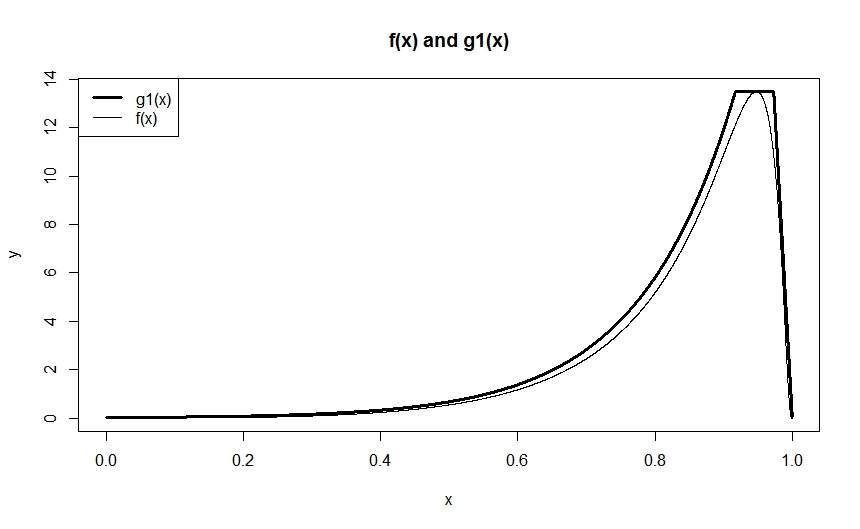
\includegraphics[scale=0.4]{1a.jpeg}
\caption{f(x) and its envelope function}
\end{figure}
\[ g_1(x) = \left\{ 
\begin{array}{l l}
e^{7.2 (x-\frac59 )} & \quad \text{for } 0 < x \leq p\\
13.5 & \quad \text{for } p < x \leq q \\
-500x+500 & \quad \text{for } q < x < 1
\end{array} \right.\]

where $p$ and $q$ are the intersection of the lines and
\begin{align*}
p &= \frac{log(13.5)}{7.2} + \frac59 \approx 0.917
\\ q &= \frac{486.5}{500} = 0.973
\end{align*}

We do a quick check on \url{R} to make sure that $g_1$ envelopes $f$ completely within the range, and indeed it does.

Now we integrate $g_1$ to find its area, then re-scale $g_1$ so that its area equals t0 1.

$$\int_0^x e^{7.2(u-\frac59)} \,du = \left[ \frac16 e^{7.2(u-\frac59)} \right]_0^x = \frac16(e^{7.2x-4}-e^{-4}) $$
$$ \int_p^x 13.5 \,du = 13.5(x-p) $$
$$ \int_q^x -500u+500 \,du = 250(q^2 - 2q - x^2 + 2x) $$

Let 
\begin{align*}
 s &= \dfrac1{7.2}(e^{7.2p-4}-e^{-4}) \approx 1.872
\\ t &= \dfrac1{7.2}(e^{7.2p-4}-e^{-4}) + 13.5(q-p) \approx 2.628
\end{align*}

The area under $g_1$ calculated analytically is 2.810163. So we define another function $g$ by $g = \frac{g_1}{2.810}$. $g$ is then a pdf which mimics the shape of $f$.

We get that $M = \sup \frac{f}{g} \approx 2.808$, and so the theoretical acceptance probability is approximately $\frac{\int f \,dx}{M} \approx 0.892$, with the integral calculated numerically using \url{R}.

The cdf, $G$, of $g$ is therefore

\[ G(x) = \left\{ 
\begin{array}{l l}
\frac1{(7.2)(2.810)}(e^{7.2x-4}-e^{-4}) & \quad \text{for } 0 < x \leq p\\
\\
\frac1{2.810}(s + 13.5(x-p)) & \quad \text{for } p < x \leq q \\
\\
\frac1{2.810}(t + 250(q^2 - 2q - x^2 + 2x)) & \quad \text{for } q < x < 1
\end{array} \right.\]

and its inverse, $G^{-1}$, is given by

\[ G^{-1}(y) = \left\{ 
\begin{array}{l l}
\frac1{7.2}(\log((7.2)(2.810)y + e^{-4})+4 ) & \quad \text{for } 0 < x \leq G(p)\\
\\
\frac{2.810y - s}{13.5} + p & \quad \text{for } G(p) < x \leq G(q) \\
\\
1 - \sqrt{1 - \frac{2.810y - t}{250} - q^2 + 2q} & \quad \text{for } G(q) < x < 1
\end{array} \right.\]

\begin{figure}[H]
\centering
	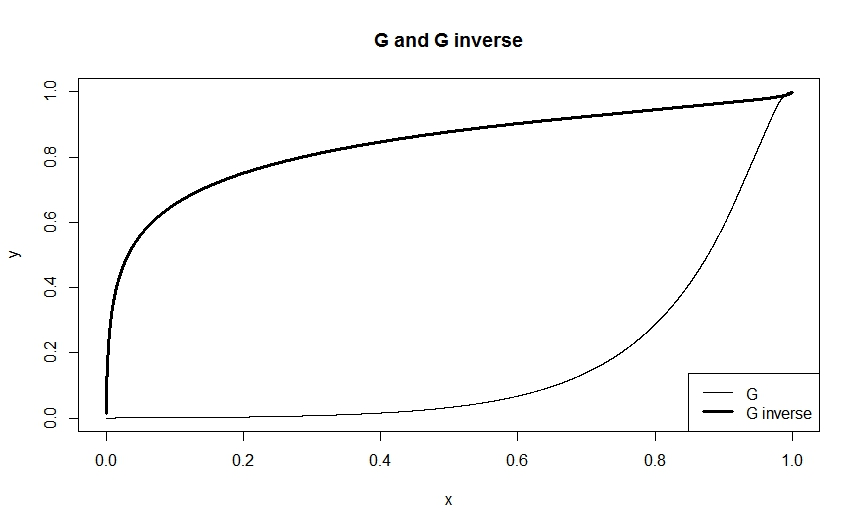
\includegraphics[scale=0.4]{1G.jpeg}
\caption{G and G inverse}
\end{figure}

\subsection{Rejection method}

We then apply the REJECTION algorithm, by first generating $y$ from $g$ using INVERSION, $u$ from the uniform distribution on (0,1), and set $x=y$ if $u \le \frac{f(y)}{Mg(y)}$, else reject $y$ and repeat the process. We apply this algorithm to generate a random sample of 1000000 and plot the histogram of our sample.

\begin{figure}[H]
\centering
	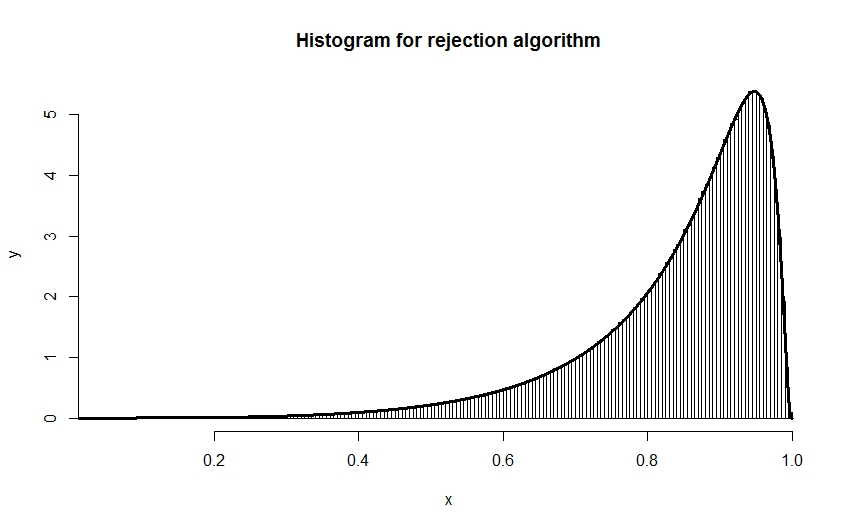
\includegraphics[scale=0.4]{1hist.jpeg}
\caption{Sample of 1000000 values}
\end{figure}

We can see that our randomly-generated sample follows the distribution of $f(x)$ very closely. The acceptance probability in practice here is 0.8928408, almost exactly the same as the theoretical acceptance probability.


\section{Monte-Carlo integration}

\subsection{Importance Sampling}

We will use the Monte-Carlo integration to approximate the area under the given $f(x)$, and hence find the normalising constant for the function. We will first use Importance Sampling, where we let

$$ \theta = \int f(x) \,dx = \int \phi(x)f(x) \,dx = \int \phi(x) \dfrac{f(x)}{g(x)} g(x) \,dx = \int \psi(x)$$

Here $\phi(x)$ is the function that restricts the integral, so $\phi(x) = 1$ if $x \in (0,1)$, 0 otherwise. $g(x)$ is some pdf. The estimate $\hat{\theta}$ is therefore

$$ \hat{\theta}_g = \frac1{n} \sum_i \psi(X_i) $$

where $X_i \sim g$.

We want to reduce the variance of $\hat{\theta}_g$ to get a more precise estimate, so we calculate the variance:
\begin{align*}
 \Var(\hat{\theta}_g) &= \frac1{n}\Var(\psi(X))
\\ &= \frac1{n} \Var \left( \phi(X) \dfrac{f(X)}{g(X)} \right)
\\ &= \frac1{n} \left(\E_g \left[ \left( \phi(X) \dfrac{f(X)}{g(X)} \right)^2 \right] - \E_g^2\left[ \phi(X) \dfrac{f(X)}{g(X)} \right]  \right)
\\ &= \frac1{n} \left( \int_0^1 \dfrac{f^2(x)}{g(x)} \,dx - \left( \int \psi(x)g(x) \,dx \right) ^2 \right)
\\ &= \frac1{n}\left( \int_0^1 \dfrac{f^2(x)}{g(x)} \,dx - \hat{\theta}_g^2 \right)
\end{align*}

We will calculate the variances numerically, so we will not use the last three lines above.

If we let $g$ be the uniform distribution on $(0,1)$, i.e. $g(x) = 1$ in this range, then we can let $\phi(x) = 1$ as all values will be within the range. The variance for $n=1000000$ is
$$ \Var(\hat{\theta}_g) = \frac1{1000000} \Var \left( \phi(X) \dfrac{f(X)}{1} \right) = \frac1{1000000} \Var ( f(X) ) \approx 1.436633 \times 10^{-5} $$

But if we let $g$ be our envelope function developed in Question 1, again $\phi(x) = 1$ as all values will be within the range. The variance for $n=1000000$ is 
$$ \Var(\hat{\theta}_g) = \frac1{1000000} \Var \left( \phi(X) \dfrac{f(X)}{g(X)} \right) = \frac1{1000000} \Var \left( \dfrac{f(X)}{g(X)} \right) \approx 6.061479 \times 10^{-8} $$

This agrees with the second line in our calculations above, where we see that we can minimise this variance by letting $ \phi(X) \frac{f(X)}{g(X)} $ be as constant as possible, and the envelope function clearly mimics the shape of $f(x)$ better than the uniform distribution. 

We will choose our envelope function in Question 1 to be our $g$. We can also generate from $g$ using the INVERSION method. We can now apply Monte-Carlo integration by generating a uniformly random sample, running it through the inverse of the cdf of $g$, and calculate $\frac1{n} \sum_i \frac{f(X_i)}{g(X_i)}$. We run the algorithm on 1000000 samples and get $\hat{\theta}_g = 2.506705$ with variance $6.061479 \times 10^{-8}$.


\subsection{Stratified Sampling}
Since our $g$ is a piece-wise function, we could potentially use Stratified Sampling, i.e. breaking up $f$ into pieces and applying Monte-Carlo to each piece. In this, case, we would break up $f$ into three pieces: one with range $(0,p]$, another with range $(p,q]$, and another with range $(q,1)$. Then $\phi(x)$ for each piece would be $\phi(x)=1$ is $x$ is in the range, 0 otherwise. $g$ for each piece would be each of the three original functions that made up the envelope function.

Running Stratified Sampling with 10000 samples on each piece of $f$ and summing them gives $\hat{\theta} = 2.506824$, which is also a good estimate. However, the variance, which in this case is the sum of the variances from each section since they're uncorrelated, is $3.093939 \times 10^{-5}$. The variance is quite high, so perhaps this method isn't the better one in this case. 

\section{Metropolis-Hastings sampler}

We will now use the Metropolis-Hastings (MH) algorithm to generate random samples from our $f(x)$. We let the continuous proposal distribution be $y = x + W$ where $y$ is the proposed new state, $x$ is the current state, $W \sim N(0,v)$, and $v$ is to be determined. Since we accept $y$ only when it falls within the range (0,1) (but not necessarily all the time when it does), the value of $v$ we choose will affect the acceptance rate.

\subsection{Tuning the parameters}

Here, there are several things we need to tune: $v$, the size of the burn-in sample, and the starting value of $x$ to use. We will start with $v$. For the sake of this selection, we let the burn-in sample be 0, and the starting value of $x$ be 0.1 as that's where $f(x)$ is small and where it would take longer to converge. Applying the MH algorithm with these inputs on a range of $v$ values 5 times and taking the averages gives us the following acceptance rates:

\begin{quote}
\begin{verbatim}
        v accept_rate
 [1,] 0.1  0.64533333
 [2,] 0.3  0.33333333
 [3,] 0.5  0.21333333
 [4,] 0.7  0.16666667
 [5,] 0.9  0.13333333
 [6,] 1.1  0.12400000
 [7,] 1.3  0.09866667
 [8,] 1.5  0.08533333
 [9,] 1.7  0.07733333
[10,] 1.9  0.07866667
[11,] 2.1  0.05600000
\end{verbatim}
\end{quote}

Since we want to keep the acceptance rate at around 20\%, we will choose $v$ to be 0.5.

Next, we see how the starting value affects the convergence of the algorithm. With 150 samples, the number of burn-ins as 0 and $v$ as 0.5, we get the following plot of sample paths for three starting values of $x$, 0.1, 0.5 and 0.9.

\begin{figure}[H]
\centering
	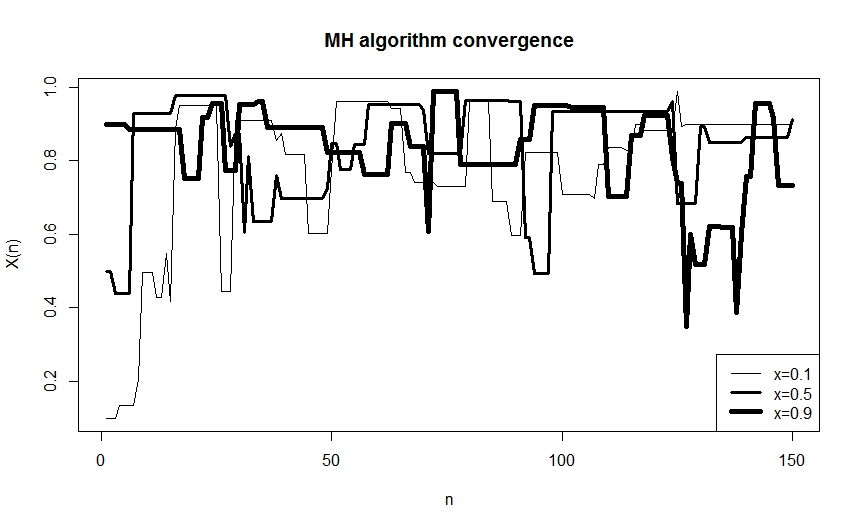
\includegraphics[scale=0.4]{3conv.jpeg}
\caption{Sample paths for different starting values}
\end{figure}

To follow the density of $f(x)$, we should be getting many more values around the 0.8-1.0 range than the rest, so we know that the algorithm converges when this happens. So for $x=0.1$, it takes about 20 samples to converge, for $x=0.5$, about 10 samples, and for $x=0.9$, about 5. The algorithm converges quicker as the starting values are higher, which is as expected, as lower values of $x$ correspond to lower values of $f(x)$, which means that the algorithm would be more likely to "miss" $f(x)$ and hence take longer to converge.

In essence, it doesn't matter which starting point we choose, so long as we adjust the burn-in sample size to reflect this. For this algorithm, we will let the starting value be 0.3. Now we plot 5 sample paths for this starting value and determine the size of burn-ins.

\begin{figure}[H]
\centering
	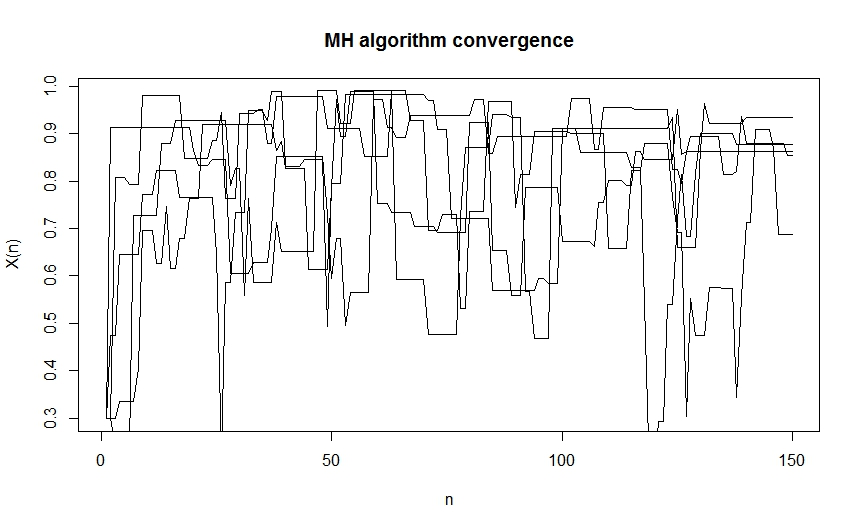
\includegraphics[scale=0.4]{3conv2.jpeg}
\caption{Sample paths for starting value 0.3}
\end{figure}

The algorithm converges at around $n=15$ for all the runs, and that doesn't change no matter how many samples we generate, so we will let our burn-in sample size be 15.

Now we will run the algorithm for 200000 samples with 15 burn-ins, $v=0.5$, and starting value at 0.3. The acceptance rate for this sample is 21.54\%. 

We then look at how it converges, by plotting and comparing histograms for the first two hundred values in the resulting sample, the next two hundred, and so on 6 times. These plots can be found in Appendix A as Figure 9.

We can see that in Figure 9a, there number of samples in the lower range and higher range are out of proportion considering our original function, but they slowly match up as we progress further, which shows the convergence for this algorithm.

\subsection{Auto-correlation sequence}
Our aim is to generate a random sample from our density $f(x)$. However, is our generated sample random? We plot an auto-correlation sequence to check that.
\begin{figure}[H]
\centering
	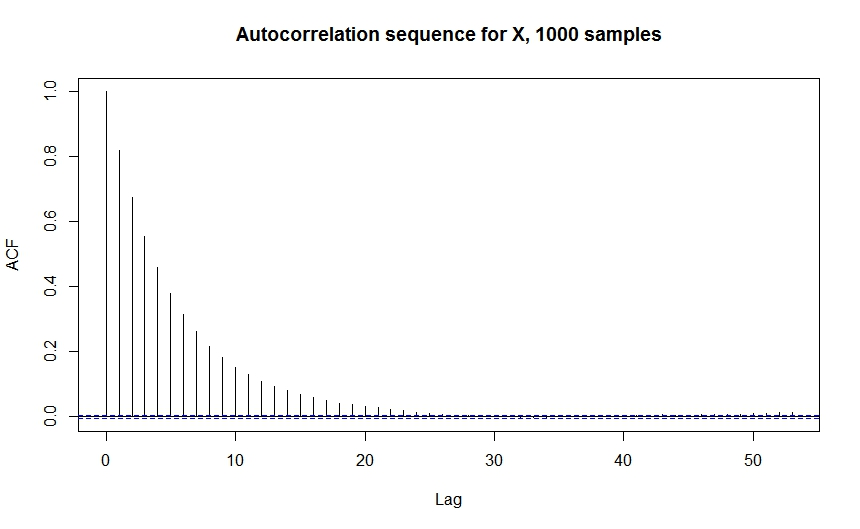
\includegraphics[scale=0.4]{3acf1.jpeg}
\caption{Auto-correlation sequence for our sample}
\end{figure}

Clearly, our sample is not random. However, the correlation drops as lag increases, and at a lag of 25 values, we can say that the correlation is negligible. So, we will create a new sample by taking every 25th value from our original sample. Now we check the auto-correlation sequence for this new sample.

\begin{figure}[H]
\centering
	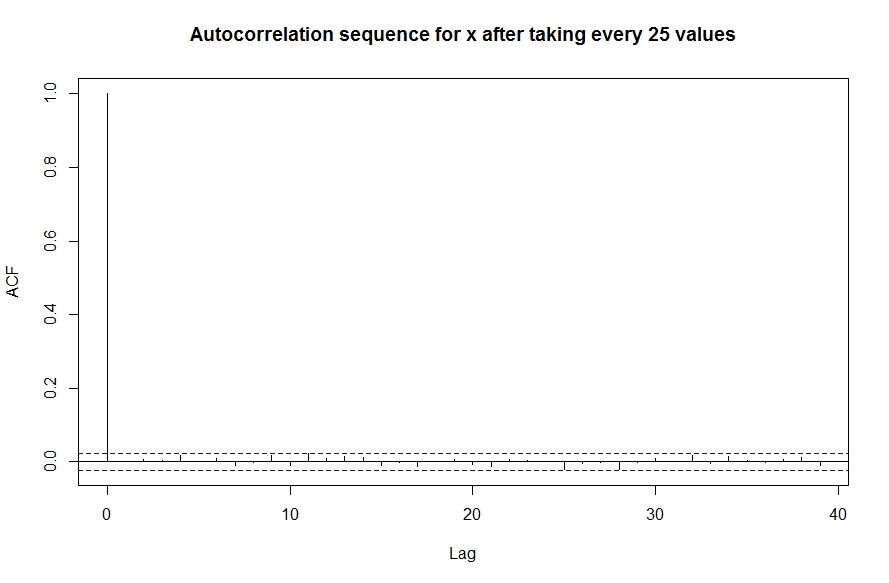
\includegraphics[scale=0.4]{3acf2.jpeg}
\caption{Auto-correlation sequence of every 25th value in the sample}
\end{figure}

It seems that our new sample is indeed uncorrelated, hence achieving our goal of generating random samples. The following plot is the density histogram of our generated new sample.

\begin{figure}[H]
\centering
	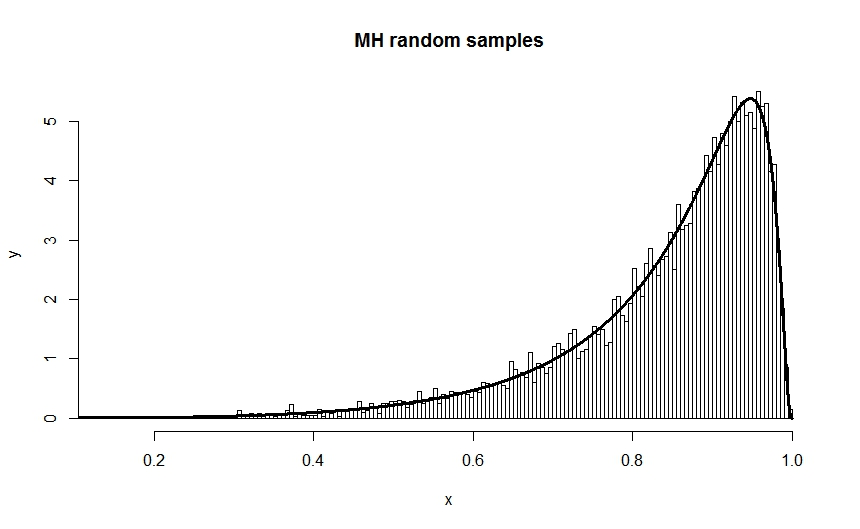
\includegraphics[scale=0.4]{3mh.jpeg}
\caption{New sample}
\end{figure}

Comparing this method to the rejection method, we can see quite clearly that the sample generated by MH algorithm doesn't adhere to our given density as well as the sample generated by rejection method. However, the advantage of the MH algorithm is that it doesn't require the use of an envelope function, hence omitting a potentially tedious step.


\newpage
\section{Appendix A: Plots}

\begin{figure}[H]
\begin{minipage}{.55\linewidth}
\centering
\subfloat[]{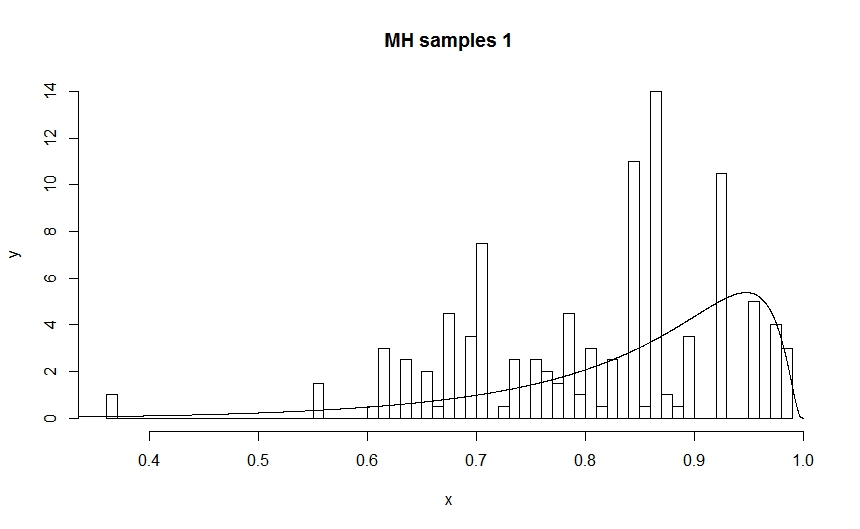
\includegraphics[scale=.25]{3mh1.jpeg}}
\end{minipage}
\begin{minipage}{.5\linewidth}
\centering
\subfloat[]{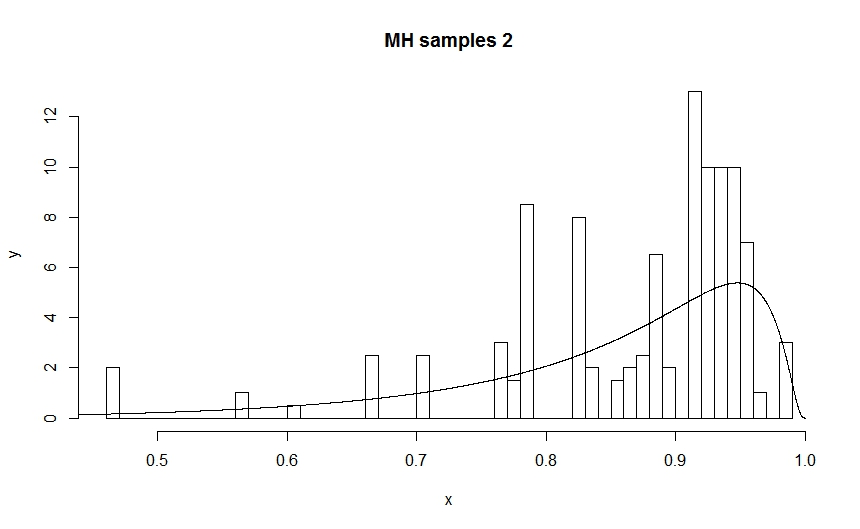
\includegraphics[scale=.25]{3mh2.jpeg}}
\end{minipage}
\begin{minipage}{.55\linewidth}\par\medskip
\centering
\subfloat[]{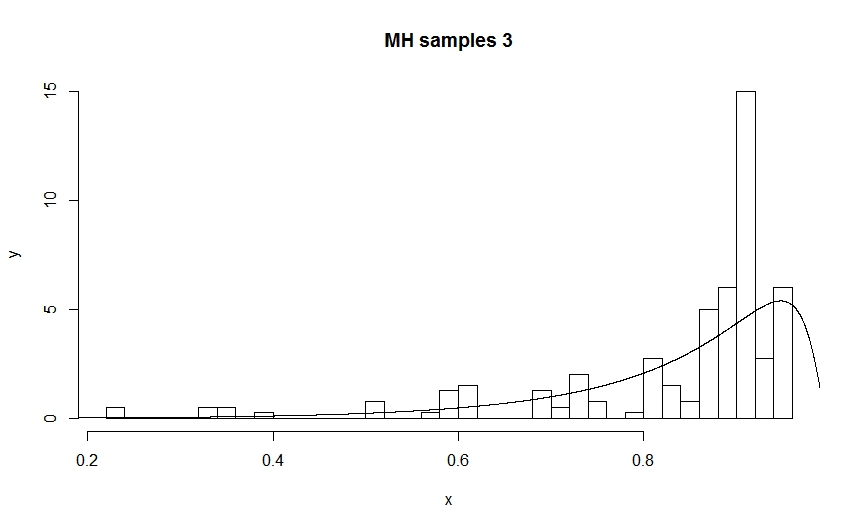
\includegraphics[scale=.25]{3mh3.jpeg}}
\end{minipage}
\begin{minipage}{.5\linewidth}
\centering
\subfloat[]{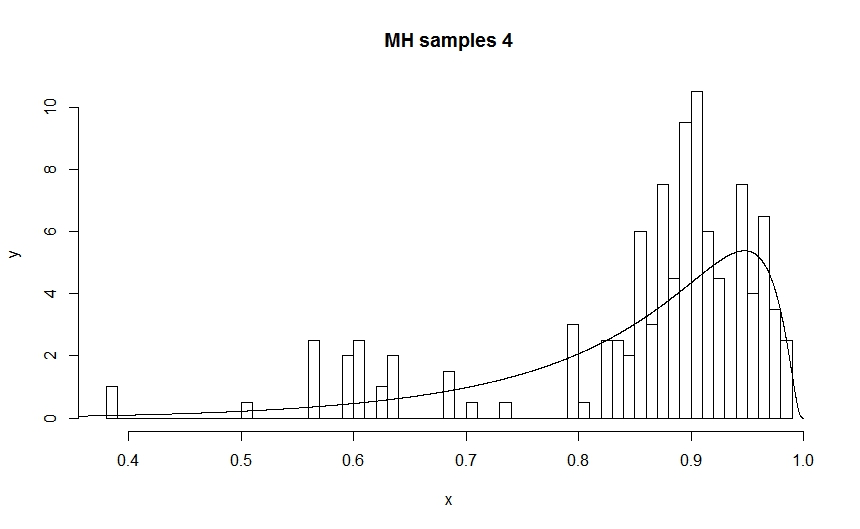
\includegraphics[scale=.25]{3mh4.jpeg}}
\end{minipage}
\begin{minipage}{.55\linewidth}\par\medskip
\centering
\subfloat[]{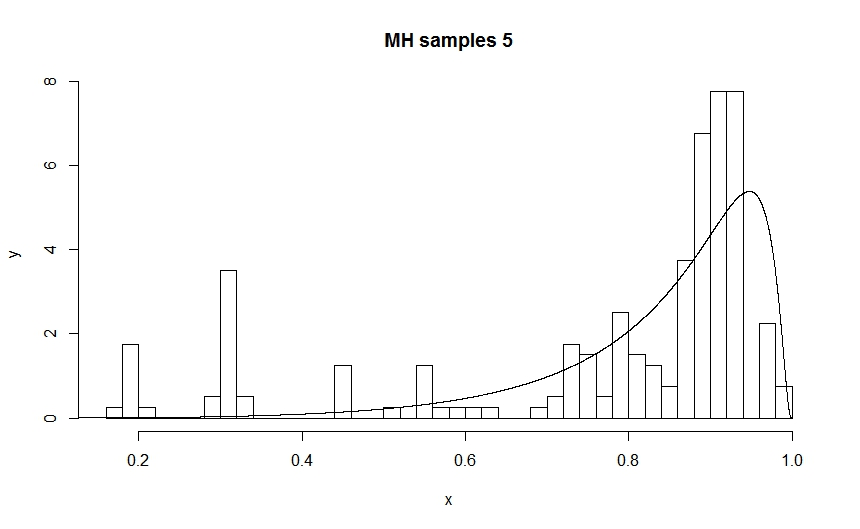
\includegraphics[scale=.25]{3mh5.jpeg}}
\end{minipage}
\begin{minipage}{.5\linewidth}
\centering
\subfloat[]{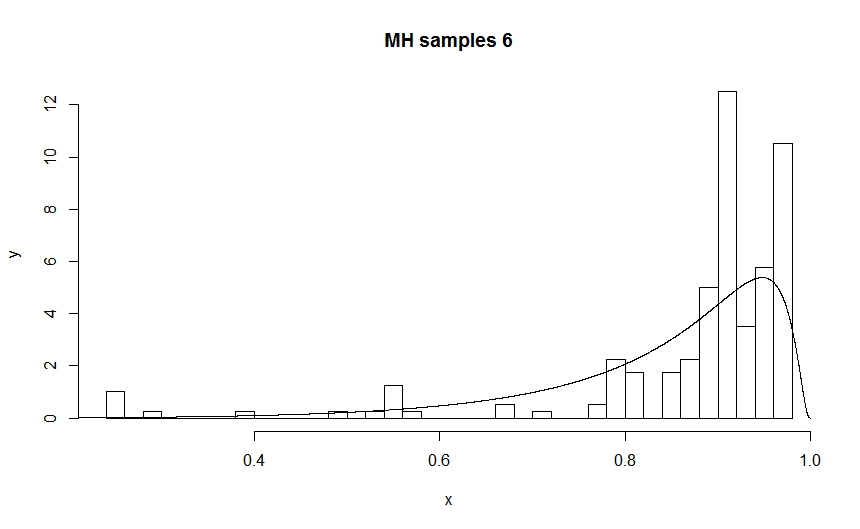
\includegraphics[scale=.25]{3mh6.jpeg}}
\end{minipage}
\caption{a) Iterations 1 to 200; b) iterations 201 to 400; c) iterations 401 to 600; d) iterations 601 to 800; e) iterations 801 to 1000; f) iterations 1001 to 1200}
\end{figure}


\newpage
\section{Appendix B: R code}

Below are the codes used in the report.

\begin{quote}
\begin{verbatim}
#' Cissy Chan
#' Stochastic Simulation Project
#' M3S9
#' March 2014

set.seed(6)

# set up target function
f <- function(x) {
  (1/(x*(1-x))) * exp((-1/2)*(-2+log(x/(1-x)))^2)
}

# visualise the target function
x <- as.matrix(seq(0, 1, length=10000)[-c(1,10000)])
fx <- apply(x, 1, f)
plot(x, fx, type="l")

# fit the envelope function on f and find their intersections
# the envelope function part 1: exponential
e <- function(x) { exp(8 * 0.9 * (x-5/9)) }
ex <- apply(x, 1, e)
lines(x, ex, type="l")

# the envelope function part 2: flat line
lx <- rep(13.5, dim(x)[1])
lines(x, lx, type="l")

# the envelope function part 3: linear
h <- function(x) { -500 * x + 500 }
hx <- apply(x, 1, h)
lines(x, hx, type="l")

# intersection points of the three pieces of the envelope function
p <- log(13.5)/(7.2) + 5/9
q <- 486.5/500

# set up the full envelope function, i.e. "g(x)" unscaled
# scale this later when we calculate its area
g1 <- function(x) {
  ifelse(x <= p, exp(7.2 * (x-5/9)), 
         ifelse(x <= q, 13.5, -500 *x + 500))
}

# plot our unscaled envelope function
g1x <- apply(x, 1, g1)
plot(
  x=x, 
  y=fx, 
  type="l", 
  main="f(x) and g1(x)",
  xlab="x", 
  ylab="y"
)
lines(x, g1x, type="l", lwd=3)
legend("topleft", legend=c("g1(x)","f(x)"),lwd=c(3,1))

# area of g1 at intersections
s <- (1/7.2) * (exp(7.2 * (p-5/9))-exp(-4))
t <- s + 13.5 * (q-p)

# area under g1
area <- t + 250 * (q^2 - 2*q + 1)

# g; rescale g1 so that area = 1
g <- function(x) {
  g1(x)/area
}

# plot g(x) scaled
gx <- apply(x, 1, g)
lines(x, gx, type="l")

# check that g1 indeed envelopes f
optimise(function(k) f(k)-g1(k), c(0,1), maximum=T)

# using optimise() on the section of the function most likely to have the supremum
# get supremum M
M <- optimise(function(k) f(k)/g(k), c(0.5,1), maximum=T)$objective

# calculate theoretical acceptance probability
ap <- integrate(f, 0, 1)$value/M
ap

# set up CDF of g
G <- function(a) {
  ifelse(a <= p, (1/area) * (1/(8*0.9)) * (exp(8*0.9*a-4) - exp(-4)),
         ifelse(a <= q, (1/area) * (s + 13.5*(a-p)),
                (1/area) * (t + 250 * (q^2 - 2*q - a^2 + 2*a))))
}

Gx <- apply(x, 1, G)

# set up inverse of CDF of g
Ginv <- function(y) {
  ifelse(y <= G(p), (log(8*0.9*area*y + exp(-4))+4) / (8*0.9),
         ifelse(y <= G(q), (area*y-s) / 13.5 + p, 
                1 - sqrt(1 - ((area*y-t) / 250 - q^2 + 2*q))))
}

y <- x

Gy <- apply(y, 1, Ginv)

# plot G and its inverse
plot(x, Gx, type="l", main="G and G inverse", ylab="y")
lines(y, Gy, type="l", lwd=3)
legend("bottomright", c("G","G inverse"), lwd=c(1,3))

#---------------------------------------------------------------------------
# Rejection method
#---------------------------------------------------------------------------

# set up rejection algorithm
generate <- function(n) {
  rand <- vector('numeric', 0)
  m1 <- 0
  naccept <- 0
  total <- 0
  while (m1 < n) {
    count <- trunc((n-m1)*1.2)
    total <- total + count
    u <- runif(count)
    y <- Ginv(runif(count))
    naccept <- naccept + length( y[(M * g(y) * u) <= f(y)])
    rand <- c(rand, y[(M * g(y) * u) <= f(y)])
    m1 <- length(rand)
  }
  cat(paste0("number accepted = ", naccept, " out of ", total, "\n"))
  cat(paste0("acceptance prob = ", format(naccept/total),"\n"))
  rand[1:n]
}

# plot generated sample
hist(
  generate(1000000),
  breaks=150,
  freq=FALSE,
  main="Histogram for rejection algorithm",
  ylab="y",
  xlab="x"
)
lines(x, fx/2.506628)

#---------------------------------------------------------------------------
# Monte-Carlo integration
#---------------------------------------------------------------------------

# generate from uniform
monte1 <- function(n) {
  x <- runif(n)
  m <- (1/n) * sum(f(x)/1)
  var <- (1/n) * var(f(x)/1)
  result <- list(m=m, var=var)
}

# generate from envelope from before (Ginv function)
monte2 <- function(n) {
  r <- runif(n)
  x <- Ginv(r)
  m <- (1/n) * sum(f(x)/g(x))
  var <- (1/n) * var(f(x)/g(x))
  result <- list(m=m, var=var)
}

# generate samples from both methods
set.seed(6)
m1 <- monte1(1000000)
m2 <- monte2(1000000)

# variance reduction
m1$var
m2$var

# MC integration of f
m2$m

# stratified sampling: testing different functions for phi
phi1 <- function(x) { ifelse(x <= p,1,0) }
phi2 <- function(x) { ifelse(x > p & x <= q,1,0) }
phi3 <- function(x) { ifelse(x > q,1,0) }

ss1 <- function(n) {
  r <- runif(n)
  x <- Ginv(r)
  m <- (1/n) * sum(phi1(x) * f(x)/g(x))
  var <- (1/n) * var(phi1(x) * f(x)/g(x))
  result <- list(m=m, var=var)
}

ss2 <- function(n) {
  r <- runif(n)
  x <- Ginv(r)
  m <- (1/n) * sum(phi2(x) * f(x)/g(x))
  var <- (1/n) * var(phi2(x) * f(x)/g(x))
  result <- list(m=m, var=var)
}

ss3 <- function(n) {
  r <- runif(n)
  x <- Ginv(r)
  m <- (1/n)* sum(phi3(x) * f(x)/g(x))
  var <- (1/n) * var(phi3(x) * f(x)/g(x))
  result <- list(m=m, var=var)
}

# generate stratified samples
set.seed(5)
s1 <- ss1(100000) 
s2 <- ss2(100000) 
s3 <- ss3(100000)

s1$m + s2$m + s3$m
s1$var + s2$var + s3$var

#---------------------------------------------------------------------------
# Metropolis-Hastings sampler
#---------------------------------------------------------------------------

# set up algorithm
mh <- function(n_sim, burn_in, starting_point, v) {
  total <- 0
  # initialixe the chain
  X <- rep(starting_point, n_sim)
  for (i in 2:n_sim) {
    Y <- X[i-1] + rnorm(1,0,v)
    ifelse(Y>0 && Y<1, alpha <- f(Y)/f(X[i-1]), alpha <- 0)
    # generate uniform random sample for probability alpha occurring
    u <- runif(1)
    X[i] <- X[i-1] + (Y - X[i-1]) * (u<alpha)
    if (i>burn_in) {total <- total + as.numeric(u<alpha)}
  }
  accept_rate <- total / (n_sim - burn_in)
  X <- X[(burn_in+1):n_sim]
  result <- list(ar = accept_rate,x = X)
}

# how v affects acceptance rates
set.seed(1)
ar <- apply(as.matrix(seq(0.1,2.1,0.2)), 1, function(x) { mh(150,0,0.1,x)$ar })
ar2 <- apply(as.matrix(seq(0.1,2.1,0.2)), 1, function(x) { mh(150,0,0.1,x)$ar })
ar3 <- apply(as.matrix(seq(0.1,2.1,0.2)), 1, function(x) { mh(150,0,0.1,x)$ar })
ar4 <- apply(as.matrix(seq(0.1,2.1,0.2)), 1, function(x) { mh(150,0,0.1,x)$ar })
ar5 <- apply(as.matrix(seq(0.1,2.1,0.2)), 1, function(x) { mh(150,0,0.1,x)$ar })
cbind(v=seq(0.1, 2.1, 0.2), accept_rate=(ar+ar2+ar3+ar4+ar5)/5)

# plots showing convergence with different starting points
set.seed(5)
v <- 0.5
plot(
  seq(1, 150),
  mh(150, 0, 0.1, v)$x,
  type="l",
  main="MH algorithm convergence",
  xlab="n",
  ylab="X(n)"
)
lines(seq(1, 150), mh(150, 0, 0.5, v)$x, lwd=3)
lines(seq(1, 150), mh(150, 0, 0.9, v)$x, lwd=5)
legend("bottomright", c("x=0.1","x=0.5","x=0.9"), lwd=c(1,3,5))

# plots showing convergence with c = 0.3 to find burn-in number
set.seed(5)
c <- 0.3
plot(
  seq(1, 150),
  mh(150, 0, c, v)$x,
  type="l",
  main="MH algorithm convergence",
  xlab="n",
  ylab="X(n)"
)
lines(seq(1, 150), mh(150, 0, c, v)$x)
lines(seq(1, 150), mh(150, 0, c, v)$x)
lines(seq(1, 150), mh(150, 0, c, v)$x)
lines(seq(1, 150), mh(150, 0, c, v)$x)

# generate auto-correlation sequence
set.seed(5)
a <- mh(200000, 15, c, v)
a$ar
acf(a$x, main="Autocorrelation sequence for X, 1000 samples")
hist(a$x[1:200], breaks=50, freq=FALSE, main="MH samples 1", xlab="x", ylab="y")
lines(x, fx/2.5066)
hist(a$x[201:400], breaks=50, freq=FALSE, main="MH samples 2", xlab="x", ylab="y")
lines(x, fx/2.5066)
hist(a$x[401:600], breaks=50, freq=FALSE, main="MH samples 3", xlab="x", ylab="y")
lines(x, fx/2.5066)
hist(a$x[601:800], breaks=50, freq=FALSE, main="MH samples 4", xlab="x", ylab="y")
lines(x, fx/2.5066)
hist(a$x[801:1000], breaks=50, freq=FALSE, main="MH samples 5", xlab="x", ylab="y")
lines(x, fx/2.5066)
hist(a$x[1001:1200], breaks=50, freq=FALSE, main="MH samples 6", xlab="x", ylab="y")
lines(x, fx/2.5066)

# auto-correlation sequence after taking every 25 values
acf(
  a$x[seq(1, length(a$x), 25)],
  main="Autocorrelation sequence for x after taking every 25 values"
)

hist(
  a$x[seq(1, length(a$x), 25)],
  breaks=150, 
  freq=FALSE,
  main="MH random samples",
  xlab="x",
  ylab="y"
)

lines(x, fx/2.5066, lwd=3)
\end{verbatim}
\end{quote}

\end{document}